\section{Dataset Construction}

The primary goal of our \DatasetName~ is to collect diverse scenes in daily life containing dense text. 
However, acquiring high-quality real-world world text-rich data is both expensive and time-consuming. 
To balance quality and scalability, we first construct \textit{Synthetic Image Split} with widely-used topics, providing easier cases for model training and evaluation.
Further, we collect \textit{Real Image Split} from diverse sources, including PowerPoint presentations, documents, existing long sequence data, and visually appealing real-world images.
By combining these tiers, \DatasetName~ provides a comprehensive and scalable resource for dense text rendering.


\begin{figure*}[h]
    \centering
    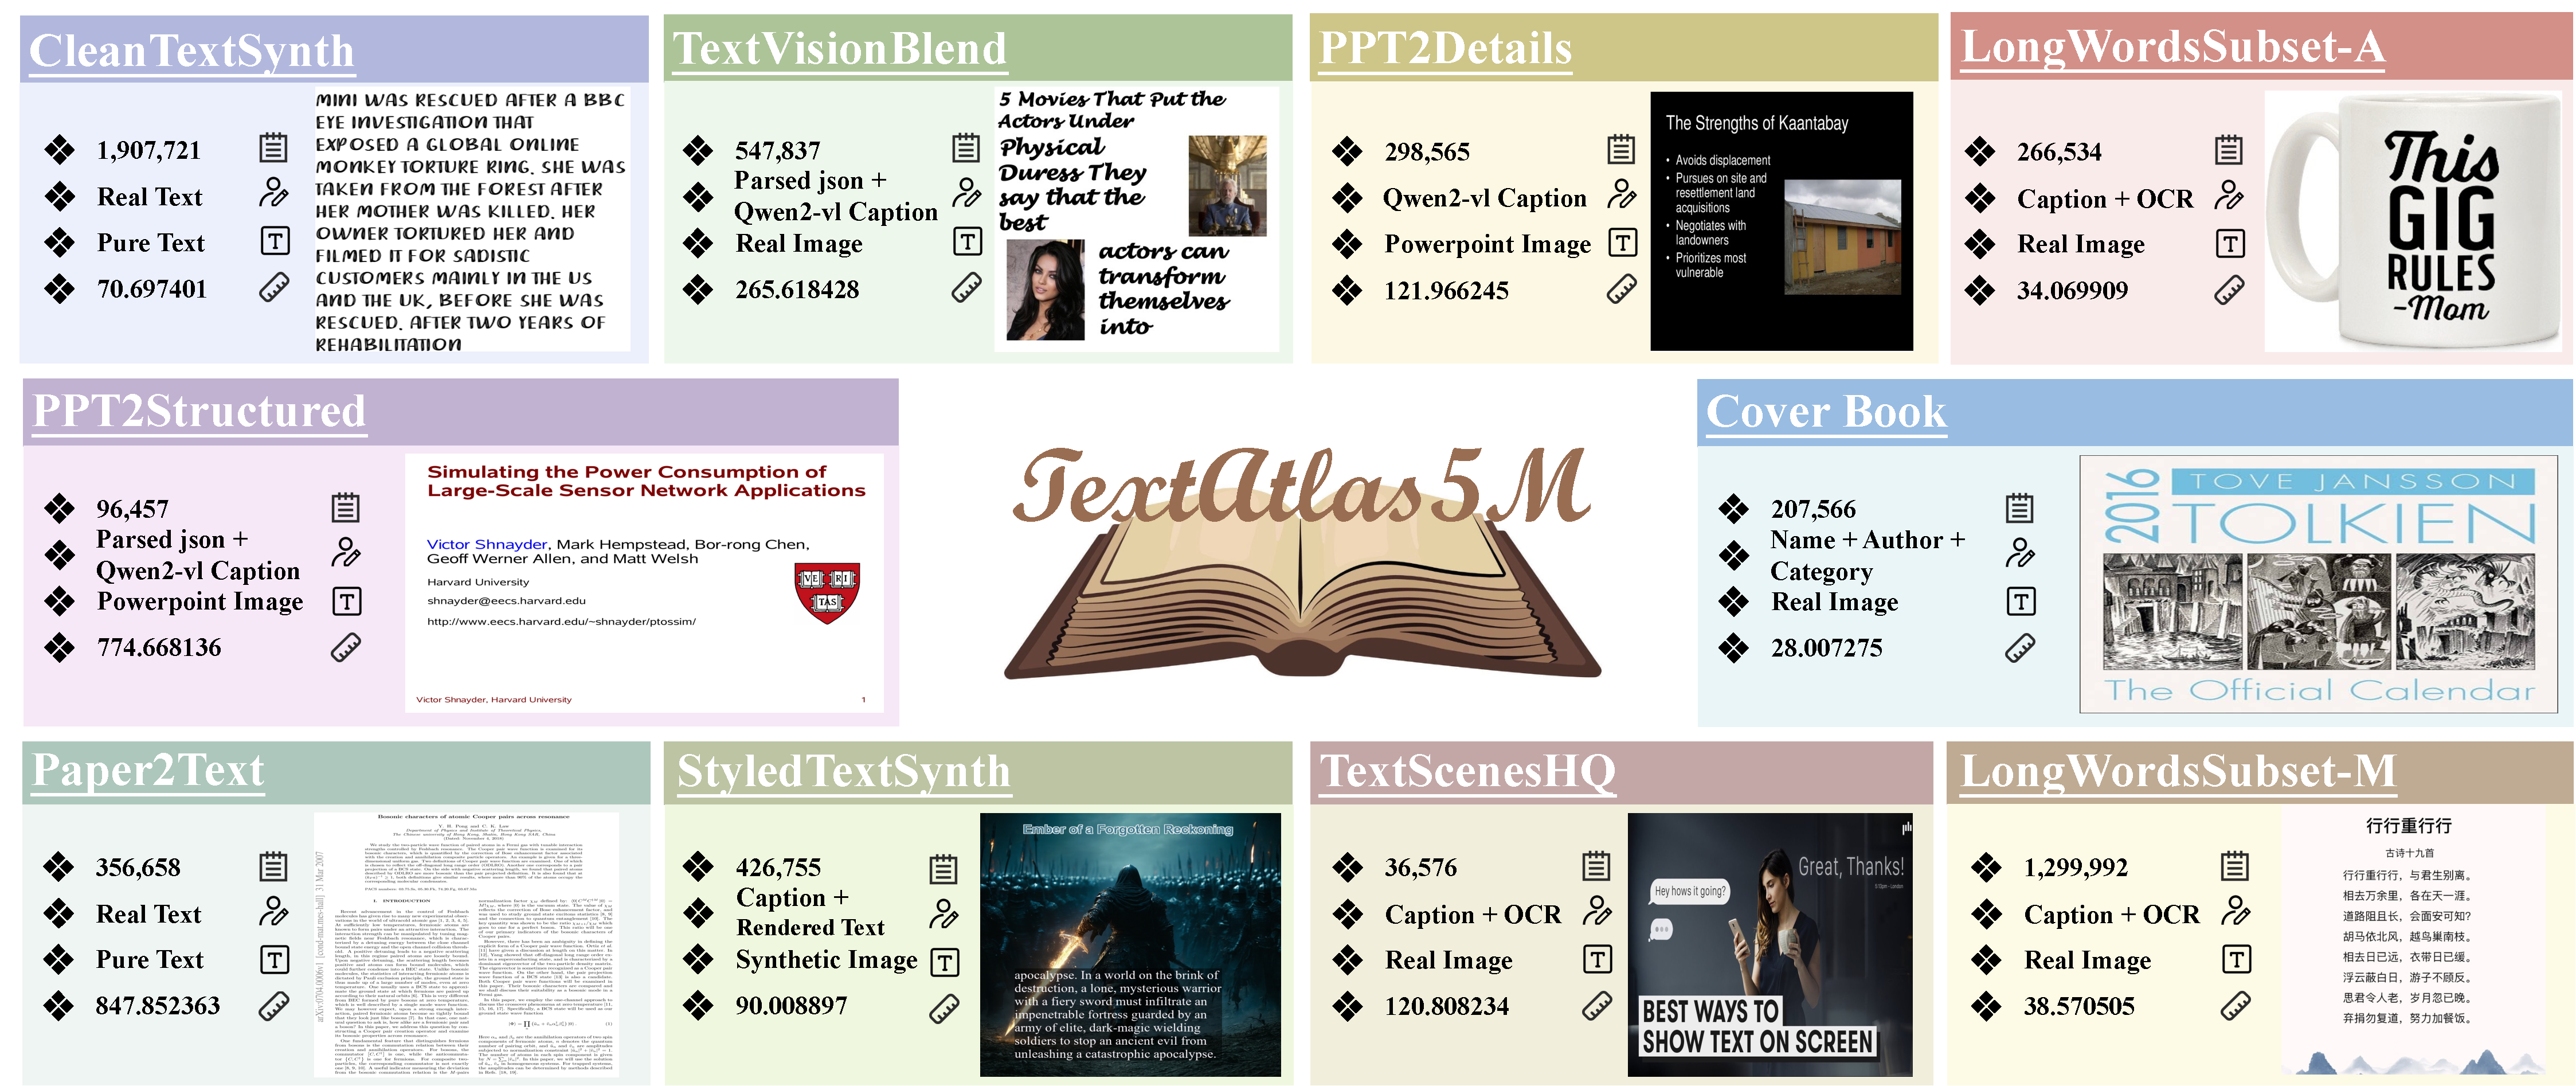
\includegraphics[width=\linewidth]{figures/src/intro_dataset.pdf}
    % \vspace{-4mm}
    \caption{
    \textbf{Overview of \DatasetName Subsets.} 
    \DatasetName\ comprises both Synthetic and Real data splits. 
    The synthetic split features three stages of increasing complexity, from clean text overlays to naturalistic text-image compositions. 
    The real-world split is sourced from a diverse set of domains, capturing authentic dense-text scenarios for robust model evaluation.
    % \textcolor{blue}{Add multi-ling example here.}
    % \textbf{Examples of Subsets in \DatasetName.}
    % The dataset includes Synthetic Data and Real Data splits. 
    % Synthetic data consists of three progressively complex subsets, while real data is gathered from diverse sources.
    }
    % \vspace{-2em}
    \label{fig:all_datasets_visualization}
\end{figure*}

\subsection{Synthetic Images Split}


\paragraph{CleanTextSynth:}
We create a simple dataset of text-only images, without incorporating additional visual elements, using the interleaved Obelics~\cite{obelics}, in which we randomly sample text sequences of length $L$.
Using OCR Rendering~\cite{ocr_rendering} for text rendering, we place sequences on white canvases with 8,700 diverse font types (e.g., Helvetica, Times New Roman). 
We introduce significant variation in font size, font color, rotation angles, and text alignment to approximate the diversity of real-world visual text while retaining control over label quality.
This results in 2 million samples of clean, well-formatted text, ideal for foundational experiments.


% Crafting Context-Rich Interleaved Data.
\textbf{TextVisionBlend: }
Interleaved data seamlessly blends visual and textual elements in formats like blogs, wikis, and newspapers. Inspired by this, we created a synthetic interleaved image-text dataset that enhances data organization and contextual richness.
We source high-quality image-text pairs from Obelics~\cite{obelics} and WIT~\cite{wit}, then design random layouts to automatically combine them. 
Using PyMuPDF~\cite{pymupdf}, we generate white-background images and parseable PDFs, ensuring structured interleaved content. From these PDFs, we extract detailed annotations, including bounding boxes, font styles, and sizes, enriching each sample.
To enhance contextual richness, we used vision-language models Qwen2-VL~\cite{qwen2_vl} and BLIP~\cite{blip} to generate image captions, consolidating all annotations and captions into comprehensive sample files. 
This dataset captures the complexity of interleaved data and see Supplementary material for more details.
% See Supplementary material \ref{sec:interleave} for details.

\paragraph{StyledTextSynth:}
Building on pure-text images and interleaved text-image scenes, we address more complex embedded text scenarios, such as billboards, to enhance dataset diversity. The overall pipeline is shown in Figure~\ref{fig:middle_quality_ppl}.
Using GPT4o~\cite{gpt4o} as a world simulator, we identify 50 real-world text-integration scenes, refining them into 18 high-frequency topics (e.g., urban signage, product packaging). GPT4o generates scene descriptions, which serve as prompts for SD3.5 to create text-free images. We then identify suitable text placement areas, refining them with human annotations as needed.
Next, LLMs like GPT4o and Llama3.1~\cite{llama3h} generate contextually relevant text, which is rendered into designated regions, producing fully annotated images aligned with each topic. 
See Appendix~\ref{sec:appendix_create_synthetic} for details on prompting and rendering.
% See Appendix~\ref{sec:appendix_create_mq} for details on prompting and rendering.



\subsection{Real Images Split}

\paragraph{PPT2Details:}
We first consider PowerPoint presentations, a widely used and text-rich format.
SlideShare1M~\cite{araujo2016slideshare} containing 1 million PowerPoint slides in an interleaved format, with most slides featuring dense text.
To annotate this dataset, we utilize Qwen2-VL~\cite{qwen2_vl}. 
The text prompt is given in Appendix~\ref{sec:appendix_template_details}.
Each slide is first converted into an image, and the model is then used to generate detailed descriptions of the text, images, and other elements, such as diagrams, tables, and vectors from this image.
To ensure high-quality annotations, we filter out slides without text and those of low quality. 
After this process, we retain a total of 0.3 million high-quality samples, providing a rich resource for further analysis and modeling.


\textbf{PPT2Structed:}
In addition to PPT2Details, we further access detailed slide elements with bounding box annotations for high-quality PowerPoint presentations. 
The AutoSlideGen dataset~\cite{autoslidegen} comprises 5,000 slides derived from scientific papers, where presentations are crafted to effectively convey research innovations.
To build this dataset, we process each slide using PyMuPDF~\cite{pymupdf} to extract element bounding boxes and their corresponding text content. 
For slides containing images, we leverage the Qwen2-VL~\cite{qwen2_vl} model to generate descriptive captions. Text elements are preserved in their raw form to maintain accuracy and context.
This process produces a structured dataset of 96,000 annotated samples, providing detailed elements along with their positional information.

\paragraph{Paper2Text:}
Another prominent text-rich scene is PDF documents, such as Arxiv papers. 
Using the Arxiv Paper dataset~\cite{arxiv_org_submitters_2024}, we process each page by extracting its content with PyMuPDF. 
For this subset, we focus primarily on text information. 
Specifically, we retain attributes such as font color, size, and type. 
This approach enables the creation of detailed annotations containing comprehensive descriptions of the text elements on each page.

\begin{wrapfigure}{r}{0.6\textwidth}
    \vspace{-1.2em}
    \centering
    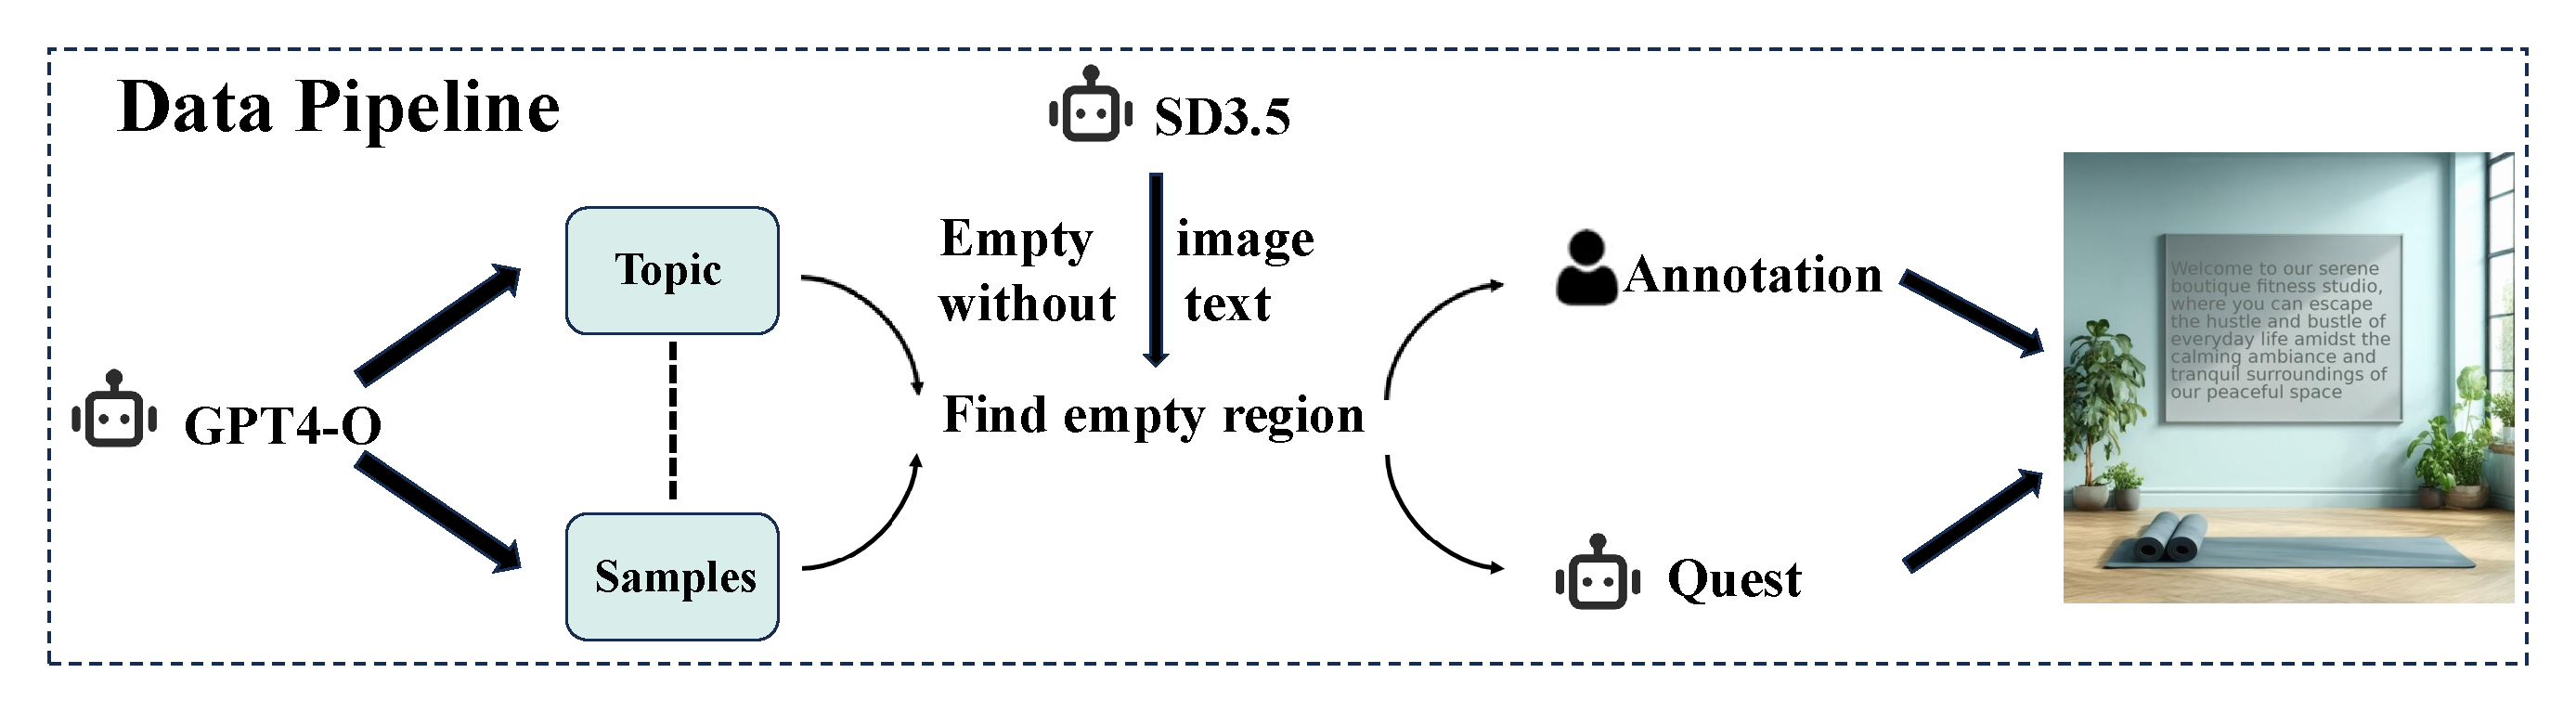
\includegraphics[width=0.58\textwidth]{figures/src/pipeline_mid.pdf}
    % \vspace{-1.5em}
    \caption{
    \textbf{StyledTextSynth Generation Pipeline.}
    GPT-4o~\cite{gpt4o} generates diverse text prompts, and a text-to-image model renders them into designated regions with seamless visual-text integration.
    }
    \label{fig:middle_quality_ppl}
    \vspace{-1.5em}
\end{wrapfigure}

% \begin{figure}
%     \centering
%     \includegraphics[width=.8\linewidth]{figures/src/MQpipeline.png}
%     \caption{
%     \textbf{StyledTextSynth Generation Pipeline.} 
%     GPT-4o~\cite{gpt4o} produces diverse text prompts, and a text-to-image model renders them into designated regions with seamless visual-text integration.
%     }
%     \label{fig:middle_quality_ppl}
% \end{figure}



\paragraph{CoverBook:}
We utilize the Cover Book dataset~\cite{coverbook}, sourced from Amazon and Inc. marketplaces. 
This dataset comprises 207,572 books spanning 32 diverse categories, with each book providing a cover image, title, author, and category information.
To create rich captions, we concatenate the title, author, category, and year information for each book.

\textbf{LongWordsSubset:}
A straightforward approach to obtain long-text samples is to filter existing text-rich image datasets. For this purpose, we use two widely adopted text rendering benchmarks: AnyWords3M~\cite{anytext} and Marion10M~\cite{textdiffuser2}.
Since most samples in these datasets contain short text, we apply a filtering process to select samples with longer words. 
The resulting subsets are named LongWordsSubset-A (from AnyWords3M) and LongWordsSubset-M (from Marion10M).
To ensure data quality, we remove duplicates, repetitive patterns, and invalid text, retaining high-quality multilingual dataset samples.
Detailed descriptions of the filtering process are shown in the Appendix~\ref{sec:appendix_create_real}.

\textbf{TextScenesHQ:}
To create a diverse and high-quality text-rich image dataset, we developed TextScenesHQ. 
Similar to StyledTextSynth, we use GPT4o as a world simulator to generate 26 predefined topics rich in text content. 
The overall pipeline is illustrated in Figure~\ref{fig:high_quality_ppl}.
The process begins with the retrieval images aligned with the specified topics from Common Crawl~\cite{mmc4}. 
These images are then filtered using OCR-based filtering rules to select those containing long text. 
Images that do not meet this threshold undergo manual screening, during which we identify candidates for enhancement, such as adding text to advertisement backgrounds to enrich their visual complexity.

After cleaning, we annotate the images using advanced models Qwen2-VL~\cite{qwen2_vl} and Intern-VL2~\cite{internvl}. 
These models generate detailed textual descriptions and bounding boxes for detected text regions. 
To ensure annotation quality, we validate them through semantic similarity checks using LLM, ensuring consistency and relevance.
For contrastive data and complex layout images, \textit{we incorporate human annotations to re-label the corresponding text to improve the data quality}.
Finally, the curated images and their validated annotations are organized into a comprehensive dataset, providing a robust resource for training and evaluation.
% See supplementary material for more details.
% See Appendix~\ref{sec:appendix_textsceneshq_annotation} for more details.


\subsection{\EvalDatasetName Generation}

To rigorously evaluate dense-text image generation, we construct \EvalDatasetName, a human-refined benchmark of 4,000 samples covering diverse domains and difficulty levels. 
We adopt a stratified sampling strategy: 1,000 samples each from StyledTextSynth, TextScenesHQ, and TextVisionBlend, representing synthetic, professional, and web-sourced interleaved scenarios. For CleanTextSynth, we sample 1,000 text instances from Obelics and apply character-level truncation at 64, 128, 256, 512, and 1024 characters to \textbf{simulate increasing complexity}.
For StyledTextSynth and TextScenesHQ, we sample uniformly across topics to ensure coverage. For TextVisionBlend, random sampling captures both controlled and organic scenes. All samples are manually refined to improve OCR accuracy and layout quality. 
Crucially, each image-text pair is \textbf{human-verified to guarantee that the image can be faithfully and completely generated from its corresponding prompt}.


\subsection{Unified Multimodal Data Construction}

A major challenge in building \DatasetName\ is unifying heterogeneous annotations across sub-datasets. 
Most samples include either scene-level descriptions or rendered text, while some also provide fine-grained attributes like bounding boxes and font sizes. 
We define a unified representation combining scene context ($S$) and rendered text content ($T$), which forms the basis for long-text image generation.

\begin{wrapfigure}{r}{0.5\textwidth}
    \vspace{-1.5em}
    \centering
    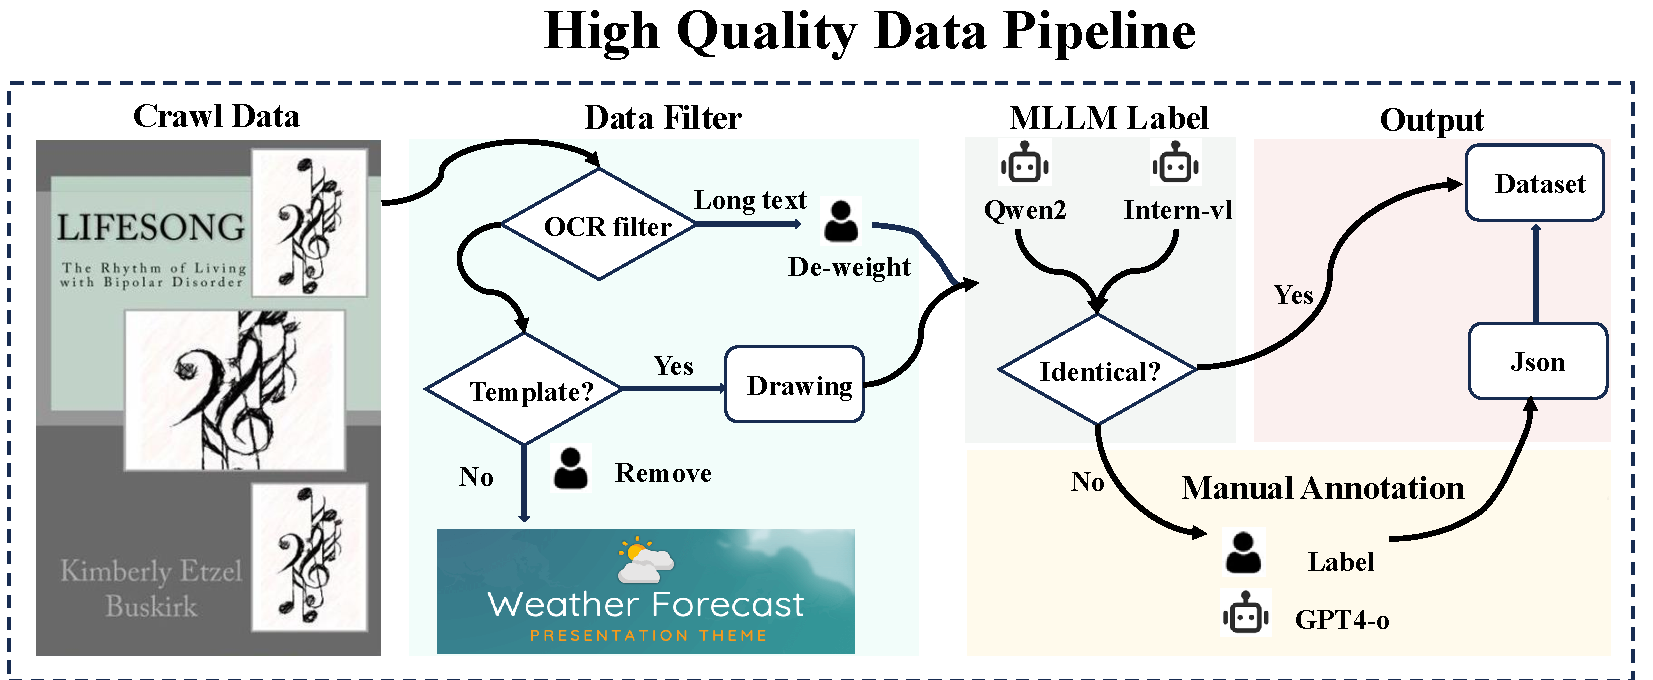
\includegraphics[width=0.48\textwidth]{figures/src/hqpipeline_fig4.pdf}
    % \vspace{-1.5em}
    \caption{
    \textbf{TextScenesHQ Generation Pipeline.}
    Data is filtered using OCR  and refined manually to correct inconsistencies from VLM.
    }
    \label{fig:high_quality_ppl}
    \vspace{-1.5em}
\end{wrapfigure}


% \begin{figure}
%     \centering
%     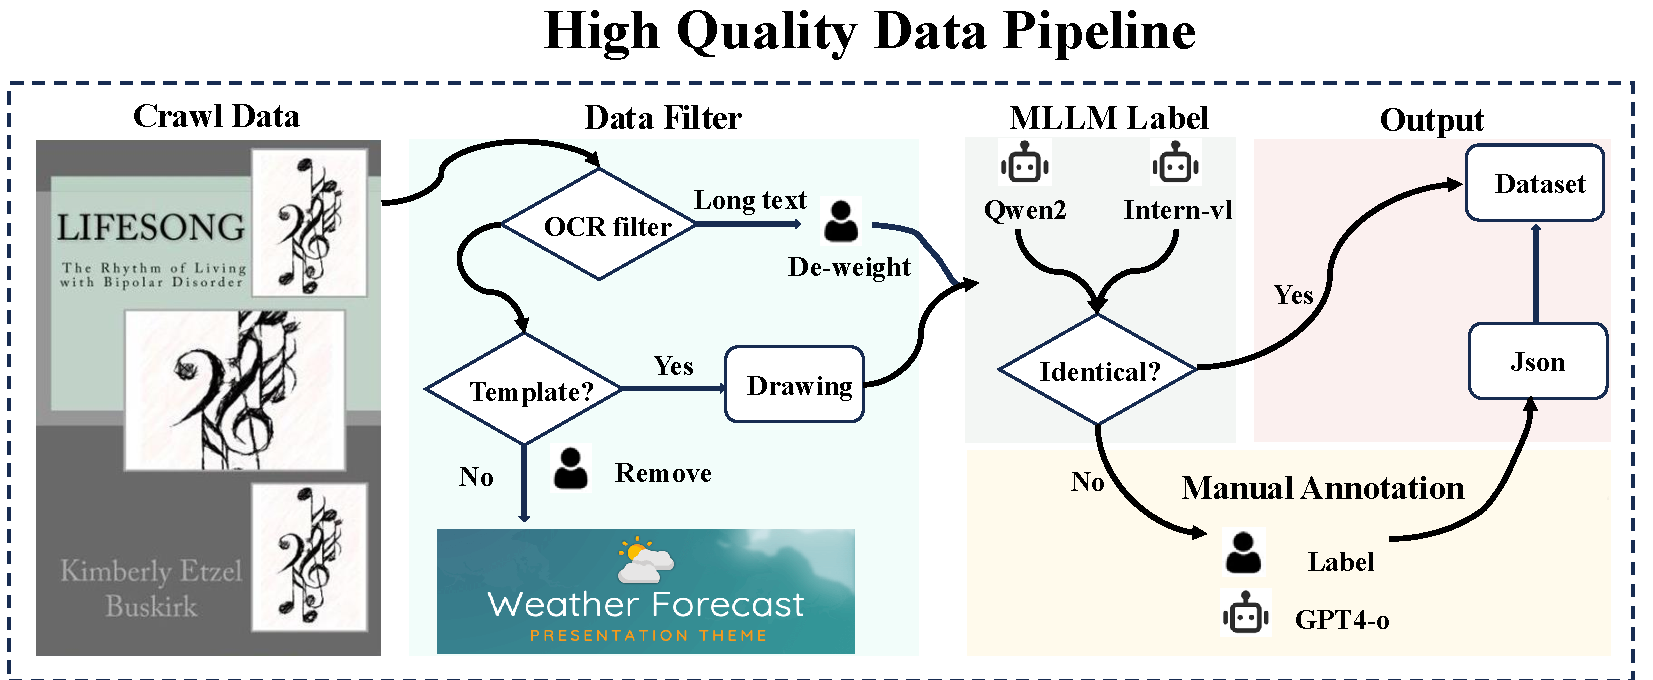
\includegraphics[width=.85\linewidth]{figures/src/hqpipeline_fig4.pdf}
%     \caption{
%     \textbf{TextScensHQ Generation Pipeline.}
%     The data is filtered using OCR results and manual annotation with correcting inconsistencies from vision-language models.
%     % The raw data undergoes rigorous filtering based on OCR rules to ensure quality. Additionally, manual annotation is applied to address inconsistencies in annotations from existing large-scale vision-language models.
%     }
%     \label{fig:high_quality_ppl}
% \end{figure}



To generate natural and coherent inputs, we leverage LLMs with adaptive prompting strategies tailored to each subset. For example, in LongWordsSubset, the LLM merges $S$ and $T$ into multiple diverse formulations. In StyledTextSynth, we use Qwen2-VL to generate scene captions with inserted placeholders (e.g., \textit{“A cozy classroom with a blackboard displaying \textless{}\textgreater.”}) to enable controllable text rendering. More dataset-specific strategies are detailed in the Appendix~\ref{sec:appendix_create_synthetic}.